\section{Methodology}\label{sec:method}
\begin{figure}[t]
\centering
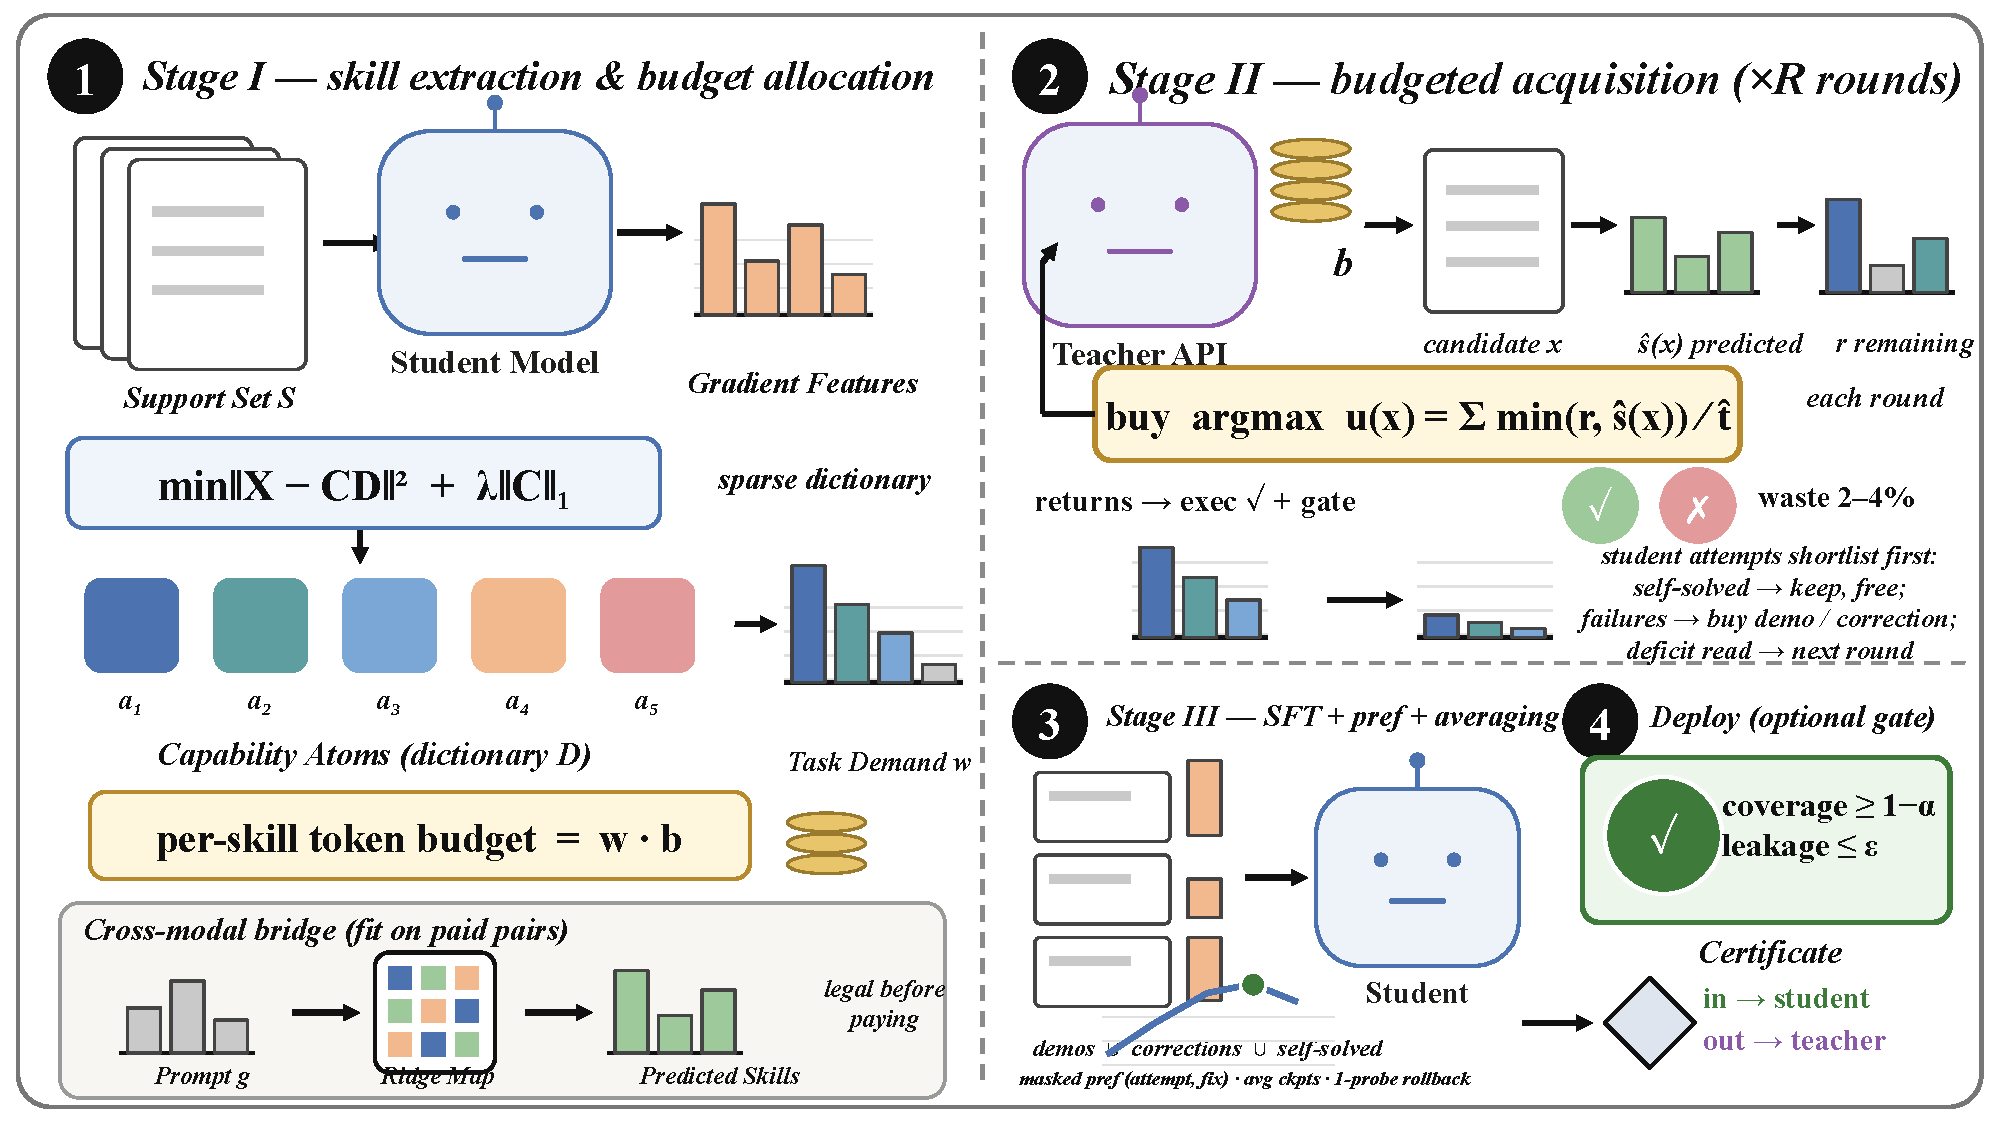
\includegraphics[width=\linewidth]{figs/fig1_mechanism.pdf}
\caption{The pipeline. One backward pass turns each example into a
gradient feature; sparse dictionary learning over these features yields
capability atoms (Definition~\ref{def:atom}), in which the support set
becomes a task demand (Definition~\ref{def:demand}) scaled to the token
budget. Acquisition queries the pay-per-token teacher where unmet demand
is largest, filters returns through an execution check and a conformal
gate, and distillation weights each admitted demonstration by the demand
it serves. The student ships with finite-sample guarantees on both sides
of the task boundary.}
\label{fig:pipeline}
\end{figure}
Figure~\ref{fig:pipeline} summarizes the pipeline. Because no training
corpus is given (Section~\ref{sec:setting}), the method cannot rank an
existing pool; it must decide what to ask the teacher, one paid query at
a time. We therefore cast few-shot distillation as \emph{active
learning against a pay-per-token teacher} \citep{settles2009active}: a
skill-level description of the task, estimated from the support set,
serves as the acquisition target; teacher queries are synthesized where
the description shows unmet need; and the returned demonstrations are
weighted, during supervised fine-tuning, by how much of that need they
serve. Concretely, one backward pass per example yields its
\emph{gradient feature} \citep{xia2024less}, a vector recording what the
student would have to learn from that example
(Section~\ref{sec:fingerprints}). Sparse dictionary learning over these
features yields \emph{capability atoms}, a task-local vocabulary of
skills, and in this vocabulary the support set induces a \emph{task
demand}: how many training tokens each skill deserves under the budget
(Section~\ref{sec:atoms}). An acquisition loop spends the budget against
this demand (Section~\ref{sec:acquire}); importance-weighted training
with behaviorally timed checkpointing turns the purchases into a student
(Section~\ref{sec:distill}); conformal calibration turns the student
into a certified, gated deployment (Section~\ref{sec:behavior}). Every
threshold is either a statistical convention ($\alpha{=}0.1$, $90\%$
mass) or estimated from the support set itself; no component is tuned
per benchmark.

\subsection{Problem setting: few-shot agent distillation}\label{sec:setting}
A task is a distribution $P_\mathcal{T}$ over queries, revealed only
through a \emph{support set} $S = \{q_1, \dots, q_k\} \sim P_\mathcal{T}$
--- the sole task-specific information any method receives. Every method
additionally gets the same three resources: a teacher agent $\pi_T$,
accessed strictly as a black-box API that returns sampled trajectories and
charges per emitted token (the regime of closed commercial models, which
rules out distribution-matching distillation \citep{gu2024minillm,
agarwal2024gkd}); an open-weight student $\theta_0$; and a token budget
$b$ capping all teacher tokens purchased over the entire run. There is no
pre-existing corpus: every demonstration must be generated by querying
$\pi_T$, every returned token is charged against $b$, and the support set
is never expanded.

From $(S, \pi_T, \theta_0, b)$ a method must produce a boundary predictor
$\hat{B}$ with distribution-free coverage
$\Pr_{q\sim P_\mathcal{T}}[\hat{B}(q)=\text{in}] \ge 1-\alpha$, and a
student evaluated two-sidedly: coverage risk (in-domain failures) and
leakage (out-of-domain capability), under matched $(S, \pi_T, b)$,
together with the budget-to-target level $B^{*}(\tau)$ and the wasted
fraction of purchased tokens. Two assumptions: \textbf{A1} the student's
gradients are accessible, and \textbf{A2} some check (executor, unit
test, judge) decides success. Code-acting agents are the instantiation we
evaluate, not a requirement.

\subsection{Gradient features: reading what an example teaches}
\label{sec:fingerprints}
Every example the method touches --- each support query, and later each
purchased demonstration --- is represented by its \emph{gradient feature}
\citep{xia2024less}: the Adam-preconditioned gradient that the example
induces on the student, compressed by a fixed random projection. The
representational point is that the gradient describes an example by what
the student would have to \emph{learn} from it, not by which words appear
in it. Identical query texts solved in two different styles are
inseparable to any function of the text, yet their gradients separate
perfectly (hard-pair AUROC $1.000$ against $0.687$ for text embeddings,
Section~\ref{sec:boundary}). Following \citet{xia2024less}, a brief
warmup on the first purchased demonstrations (four epochs, low-rank
adapter) accumulates the optimizer's second-moment statistics and absorbs
surface formatting; each example then contributes one backward pass, and
the adapter gradient is rescaled coordinate-wise by the inverse root of
the second moments, so the feature measures the update step the optimizer
would actually take. The random projection preserves the inner products
that all downstream computation consumes, up to $(1\pm\varepsilon)$
\citep{johnson1984extensions}. One distinction matters under the metered
protocol: for a purchased demonstration the feature is computed on the
teacher's response, whereas for a candidate prompt whose answer has not
been bought yet, only the feature of the \emph{prompt text} is available
--- and the acquisition step below is careful to plan with the latter and
account with the former.

\subsection{Capability atoms and task demand}\label{sec:atoms}
Gradient features of related examples are not arbitrary vectors: they
reuse a small set of recurring directions, the way recipes reuse a small
set of basic operations. Sparse dictionary learning
\citep{olshausen1996emergence} recovers exactly this structure. Writing
the feature matrix as $X$, we solve
$\min_{D,C}\ \lVert X - CD\rVert_2^2 + \lambda\lVert C\rVert_1$,
alternating a lasso step with a dictionary update.

\begin{definition}[Capability atom]\label{def:atom}
A \emph{capability atom} is one row of the learned dictionary $D$: a
unit-norm direction in gradient-feature space. The sparse code $c(x)$ of
an example $x$ is its coefficient vector over the atoms, obtained by a
lasso solve against $D$; $|c(x)|_a$ measures how strongly example $x$
exercises atom $a$.
\end{definition}

The $\ell_1$ penalty is what makes atoms identifiable, and it is the
design choice that separates this component from PCA or SVD: a subspace is
invariant to rotations of its basis, so no individual principal direction
can be identified with a skill, whereas rotating a dictionary destroys
the sparsity of its codes. The only bases that survive the penalty are
those aligned with recurring, self-contained gradient patterns --- and
those patterns behave like skills. Empirically, atom support separates
fine-grained skills within one domain at AUROC $0.906$ where the dense
subspace reaches $0.615$, and the behavioral change caused by
distillation concentrates $85.5\%$ of its mass on $5$ of $128$ atoms
(Section~\ref{sec:atoms-results}). Because no corpus is given, the
dictionary cannot be pretrained: it is fit first on the support features
alone and refit as purchased demonstrations accumulate, so the atom count
grows with the evidence, and a demonstration the current dictionary
reconstructs poorly signals, through its residual, that a new skill has
appeared.

\begin{definition}[Task demand]\label{def:demand}
Given a dictionary $D$ and the support set $S$, the \emph{task demand} is
$w = \frac{1}{k}\sum_{q\in S} |c(q)|$, normalized to sum to one and
restricted to the atoms carrying $90\%$ of its mass. Scaled by the
budget, $w \cdot b$ assigns each atom a token quota: the number of
training tokens the task asks the method to spend on that skill.
\end{definition}

The support set is a small sample, so $w$ inherits its blind spots. The
teacher's own solutions correct part of them: atoms that appear
persistently in the codes of demonstrations for support queries, yet
carry little weight in $w$, are skills the task requires \emph{implicitly}
--- the query said ``aggregate by month,'' every competent solution also
plotted --- and their demand is filled in from the demonstration side
before further budget is spent. This completion touches only how the
budget is allocated; the boundary and all certificates remain calibrated
on the original $k$ queries alone.

\subsection{Spending the budget: acquisition against demand}
\label{sec:acquire}
The acquisition loop spends $b$ against the token quotas. At each round
the method holds a set of candidate prompts (support queries, their
sampled variants in the style of self-instruct \citep{wang2023selfinstruct},
and probes), and for each candidate only its prompt-text gradient feature
is legitimately available. Encoding that feature against the current
dictionary predicts which atoms the answer would exercise; the candidate's
\emph{acquisition score} is
\[
u(x) \;=\; \frac{\sum_a \min\!\big(r_a,\ \hat{s}_a(x)\big)}{\hat{t}(x)},
\]
where $r_a$ is atom $a$'s remaining quota, $\hat{s}_a(x)$ the predicted
token contribution of $x$ to atom $a$, and $\hat{t}(x)$ the predicted
response length. The method buys the highest-scoring batch, then
reconciles: the realized response is encoded, its realized token count is
charged, and the quotas are decremented by what was actually delivered,
so prediction errors correct within a few rounds instead of compounding.
Two properties follow directly. Returns diminish endogenously: predicted
contribution beyond a filled quota counts zero, so a candidate rich in an
almost-satisfied skill loses priority with no decay constants. And
spending is auditable: every return must pass the execution check (A2)
and a conformal gate calibrated on held-out support queries
(Section~\ref{sec:behavior}); a generation that drifted off-task is paid
for --- the budget is real --- but never trains the student, and this
wasted-budget fraction is reported alongside accuracy. The contrast with
influence-based selection against a single mean target \citep{xia2024less}
is structural: collapsing a multi-skill task onto one direction leaves
surplus tokens nowhere to go but out of scope (off-task residue growing
from $0$ to $0.44$ with budget on the SQL-scoped task,
Section~\ref{sec:results}), whereas per-atom quotas give every token a
named destination. The loop stops when the quotas are filled or the
budget is exhausted; unspent budget is returned and reported, since
reaching the target cheaper is exactly the $B^{*}(\tau)$ objective.

\subsection{Distillation: the same skill vocabulary directs learning}
\label{sec:distill}
The purchased demonstrations are distilled into the student by supervised
fine-tuning, but not by uniform behavior cloning: the skill vocabulary
that directed spending now directs learning, and every departure from
plain imitation below is skill-resolved through the atoms --- the design
that separates this stage from prior agent distillation, which reweights
or corrects at the level of whole traces or states
\citep{tang2026smartad, liu2025structured, ross2011dagger}.

\textbf{Compute-matched supervised fine-tuning.} All purchased
demonstrations are distilled with standard supervised fine-tuning under a
fixed compute budget (smaller corpora receive proportionally more
epochs). We deliberately do \emph{not} reweight the loss by demand:
controlled comparisons across acquisition methods show that on
exec-verified, on-task corpora, demand weighting yields no in-task gain
and its residual boundary-control effect is subsumed by the acquisition
gate (Section~\ref{sec:experiments}); it is reported as an ablation.

\textbf{Skill-resolved absorption tracking.} Every purchased
demonstration is labeled at selection time with its dominant atom, so the
per-example training losses aggregate --- at no extra cost --- into
per-atom absorption curves: the loss trajectory of each individual skill.
These curves make the distillation process observable at the skill level:
most atoms' losses collapse within the first epochs, while a small,
seed-dependent set \emph{lags}, its purchased demonstrations failing to
teach it. Lagging skills are not treated with more epochs on data that
has already shown it cannot help; they trigger corrective acquisition.

\textbf{Skill-resolved corrective acquisition.} Half of the budget first
buys a seed corpus and trains an intermediate student. The remaining
budget is then spent \emph{against that student's deficiencies}, named in
the atom vocabulary in either of two ways: (i) the intermediate student
is rolled out on the seed prompts, execution checks flag failures, and
the failed examples' codes average into a deficit direction
(rollout-based); or (ii) the deficit is read directly from the lagging
atoms of the seed round's absorption curves, requiring no rollouts at
all (dynamics-based; the two agree in accuracy while the latter removes
the most expensive step). Candidates are ranked by their bridge-predicted
supply of the deficit and purchased until the budget closes. Where
\textsc{DAgger} \citep{ross2011dagger} forwards failure \emph{states} to
the expert and LLM2LLM \citep{lee2024llm2llm} augments near failure
\emph{instances}, the deficit here lives in skill space: correction
spreads across the deficient skill's support rather than concentrating on
hard instances, which at a matched budget buys measurably more distinct
demonstrations per token and halves the across-seed variance
(Section~\ref{sec:experiments}).

Throughout, gradient geometry is never asked to judge success: three
pre-registered experiments show it cannot (instance-level gradient
signals fail to predict success; re-selecting against residual gradients
selects noise; aggregate geometric absorption bottoms out two orders of
magnitude before behavioral competence forms,
Section~\ref{sec:mechanism}). The division of labor is strict: per-atom
demand decay only \emph{diagnoses} --- which skill is saturated, which is
stalled, where the next token should go --- while behavior remains the
sole judge of arrival. A probe every $8$ steps measures the fraction of
held-out calibration queries yielding runnable solutions, and the
best-scoring checkpoint is kept, making aggressive small-budget training
safe because drift past the competence peak is detected and rolled back.

\subsection{Certified deployment}
\label{sec:behavior}
What leaves the pipeline is not a model but a deliverable: the trained
student, a boundary predictor, and two-sided certificates. The boundary
predictor is built from the support set alone --- a subspace fit to the
gradient features of a fit split, a norm-ratio score, and a conformal
threshold from a disjoint calibration split, giving distribution-free
coverage $\ge 1-\alpha$ \citep{angelopoulos2023conformal}. The student is
then evaluated behaviorally on both sides of the boundary and the
capability match is stated as finite-sample Clopper--Pearson bounds: a
certified lower bound on in-task coverage and a certified upper bound on
off-task leakage --- a bounded claim, not a score. At deployment the same
machinery gates live requests: in-specification queries route to the
student, the rest are refused or escalated to the teacher, so the
certificates describe exactly the traffic the student will see.
